% Generated 2021-01-06 15:42:25 +0530
\subsection{Components} \label{sec:Components}


\block{Components} groups information describing physical parts or logical functions of a piece of equipment.   \block{Components} \glspl{organize} one or more \block{Component} elements. 

\begin{figure}[ht]
  \centering
    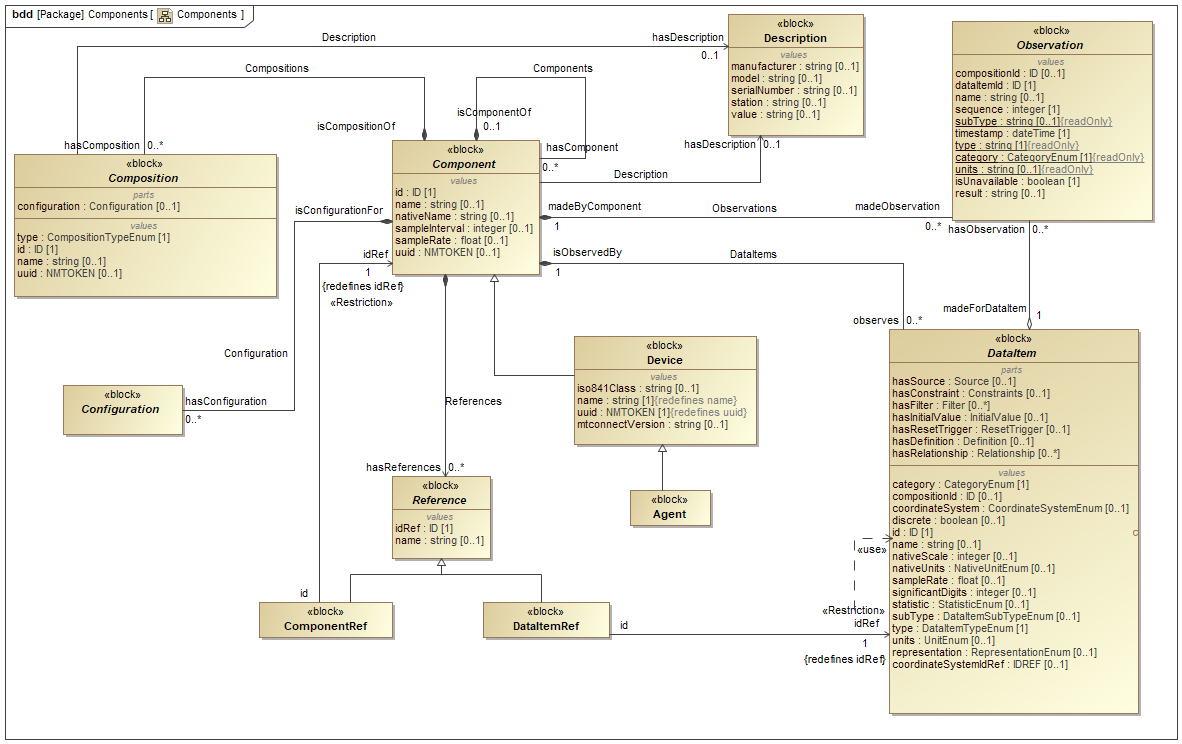
\includegraphics[width=1.0\textwidth]{figures/Components.png}
  \caption{Components Diagram}
  \label{fig:Components}
\end{figure}

\FloatBarrier



\subsubsection{Component}
\label{sec:Component}



A \block{Component} organizes information describing a physical part or logical function of a piece of equipment.


\paragraph{Attributes of Component}\mbox{}
\label{sec:Attributes of Component}

\tbl{Attributes of Component} lists the attributes of \texttt{Component}.

\begin{table}[ht]
\centering 
  \caption{Attributes of Component}
  \label{table:Attributes of Component}
\tabulinesep=3pt
\begin{tabu} to 6in {|l|l|l|} \everyrow{\hline}
\hline
\rowfont\bfseries {Attribute} & {Type} & {Multiplicity} \\
\tabucline[1.5pt]{}

\property{id}[Component] & \texttt{ID} & 1 \\
\property{name}[Component] & \texttt{string} & 0..1 \\
\property{nativeName}[Component] & \texttt{string} & 0..1 \\
\property{sampleInterval}[Component] & \texttt{integer} & 0..1 \\
\texttt{<<deprecated>>} \property{sampleRate}[Component] & \texttt{float} & 0..1 \\
\property{uuid}[Component] & \texttt{NMTOKEN} & 0..1 \\
\end{tabu}
\end{table}
\FloatBarrier

Descriptions for attributes of \block{Component}:

\begin{itemize}

\item \property{id}[Component] \newline The unique identifier for this element.

\item \property{name}[Component] \newline The name of an element or a piece of equipment.

\item \property{nativeName}[Component] \newline The common name normally associated with a piece of equipment or an element.

\item \property{sampleInterval}[Component] \newline An optional attribute that is an indication provided by a piece of equipment describing the interval in milliseconds between the completion of the reading of the data associated with the \block{Device} element until the beginning of the next sampling of that data.

\item \property{sampleRate}[Component] \newline \textbf{DEPRECATED} in \textit{MTConnect Version 1.2}. Replaced by \property{sampleInterval}[Component].

\item \property{uuid}[Component] \newline The unique identifier for an element.
\end{itemize}

\paragraph{Elements of Component}\mbox{}
\label{sec:Elements of Component}

\tbl{Elements of Component} lists the elements of \texttt{Component}.

\begin{table}[ht]
\centering 
  \caption{Elements of Component}
  \label{table:Elements of Component}
\tabulinesep=3pt
\begin{tabu} to 6in {|l|l|} \everyrow{\hline}
\hline
\rowfont\bfseries {Element} & {Multiplicity} \\
\tabucline[1.5pt]{}
\texttt{Description} & 0..1 \\
\texttt{Composition} (organized by \block{Compositions}) & 0..* \\
\texttt{Component} (organized by \block{Components}) & 0..* \\
\texttt{Configuration} & 0..* \\
\texttt{DataItem} (organized by \block{DataItems}) & 0..* \\
\texttt{Reference} (organized by \block{References}) & 0..* \\
\end{tabu}
\end{table}
\FloatBarrier


Descriptions for elements of \block{Component}:

\begin{itemize}

\item \block{Description} \newline The descriptive content.

\item \block{Compositions} \newline \block{Compositions} \glspl{organize} \block{Composition} elements.

\item \block{Components} \newline \block{Components} \glspl{organize} \block{Component} elements.

\item \block{Configuration} \newline \block{Configuration} contains technical information about a piece of equipment describing its physical layout or functional characteristics.

\item \block{DataItems} \newline \block{DataItems} \glspl{organize} \block{DataItem} elements. See \sect{DataItems}

\item \block{References} \newline \block{References} \glspl{organize} \block{Reference} elements associated with this \block{Component} element.
\end{itemize}

\subsubsection{Description}
\label{sec:Description}



The descriptive content.


The value of \texttt{Description} \MUST be \texttt{string}.


\paragraph{Attributes of Description}\mbox{}
\label{sec:Attributes of Description}

\tbl{Attributes of Description} lists the attributes of \texttt{Description}.

\begin{table}[ht]
\centering 
  \caption{Attributes of Description}
  \label{table:Attributes of Description}
\tabulinesep=3pt
\begin{tabu} to 6in {|l|l|l|} \everyrow{\hline}
\hline
\rowfont\bfseries {Attribute} & {Type} & {Multiplicity} \\
\tabucline[1.5pt]{}

\property{manufacturer}[Description] & \texttt{string} & 0..1 \\
\property{model}[Description] & \texttt{string} & 0..1 \\
\property{serialNumber}[Description] & \texttt{string} & 0..1 \\
\property{station}[Description] & \texttt{string} & 0..1 \\
\end{tabu}
\end{table}
\FloatBarrier

Descriptions for attributes of \block{Description}:

\begin{itemize}

\item \property{manufacturer}[Description] \newline The name of the manufacturer of the physical or logical part of a piece of equipment represented by this element.

\item \property{model}[Description] \newline The model description of the physical part or logical function of a piece of equipment represented by this element.

\item \property{serialNumber}[Description] \newline The serial number associated with a piece of equipment.

\item \property{station}[Description] \newline The station where the physical part or logical function of a piece of equipment is located when it is part of a manufacturing unit or cell with multiple stations.

\item \property{value}[Description] \newline The description of the element.
\end{itemize}
